%%
%% Template de TCC para os cursos EAD do Centro Universitário SENAC.
%% Desenvolvido por Daniel de Mello Viero <daniel.viero@gmail.com> em maio/2019.
%% Foi baseado no modelo DOCX fornecido pelo SENAC.
%% A estrutura está quase toda definida na classe senac-tcc.cls. Este arquivo
%% tem o conteúdo do TCC.

%% Este template e o arquivo de classe estão disponíveis para quem quiser usar,
%% mas talvez não se aplique a todos os casos. Está aberto para aprimoramento 
%% pelos interessados. Eu não tenho profundo conhecimento em Latex, sugiro 
%% consultar a ótima documentação em https://github.com/abntex/abntex2 
%% (que eu usei para criar a customização) e outras fontes na Internet.

\documentclass[]{senac-tcc}

% ---
% Pacotes adicionais, usados apenas para o template
% ---
\usepackage{lipsum}				% para geração de dummy text
% ---

% ---
% Pacotes específicos para este documento
% ---
\usepackage{pdfpages} % Para incluir PDFs prontos, como a ficha catalográfica.

% ---
% Informações de dados para CAPA e FOLHA DE ROSTO
% ---
\titulo{Título do Trabalho}
\autor{Nome do Aluno}
\curso{Nome do Curso}
\local{São Paulo}
\campus{Santo Amaro}
\data{2019}
\orientador{Nome do mediador}
%\coorientador{Nome do co-orientador, se aplicável}
\examinadores{Nome 1}{Nome 2}

% ---
% Configurações de aparência do PDF final
% ---
% alterando o aspecto da cor azul
\definecolor{blue}{RGB}{41,5,195}

% ---
% informações do PDF
% ---
\makeatletter
\hypersetup{
     	%pagebackref=true,
		pdftitle={\@title}, 
		pdfauthor={\@author},
    	pdfsubject={\imprimirpreambulo},
	    pdfcreator={LaTeX with abnTeX2},
		pdfkeywords={palavra-chave 1}{palavra-chave 2}{palavra-chave 3}, 
		colorlinks=true,       		% false: boxed links; true: colored links
    	linkcolor=blue,          	% color of internal links
    	citecolor=blue,        		% color of links to bibliography
    	filecolor=magenta,      		% color of file links
		urlcolor=blue,
		bookmarksdepth=4
}
\makeatother
% --- 

% --- 
% Espaçamentos entre linhas e parágrafos 
% --- 

% O tamanho do parágrafo é dado por:
\setlength{\parindent}{1.3cm}

% Controle do espaçamento entre um parágrafo e outro:
\setlength{\parskip}{0.2cm}  % tente também \onelineskip

% ---
% compila o indice
% ---
\makeindex
% ---

% ----
% Início do documento
% ----
\begin{document}

% Retira espaço extra obsoleto entre as frases.
\frenchspacing 

% ----------------------------------------------------------
% ELEMENTOS PRÉ-TEXTUAIS
% ----------------------------------------------------------
% \pretextual

% ---
% Capa
% ---
\imprimircapa
% ---

% ---
% Folha de rosto
% (o * indica que haverá a ficha bibliográfica)
% ---
\imprimirfolhaderosto*
% ---

% ---
% Inserir a ficha bibliografica
% ---

% Gere um arquivo PDF da ficha catalográfica no site da Biblioteca do SENAC, 
% no link http://www.sp.senac.br/jsp/default.jsp?template=2202.dwt&testeira=386.
% Substitua o arquivo exemplo usado aqui.
%
\begin{fichacatalografica}
    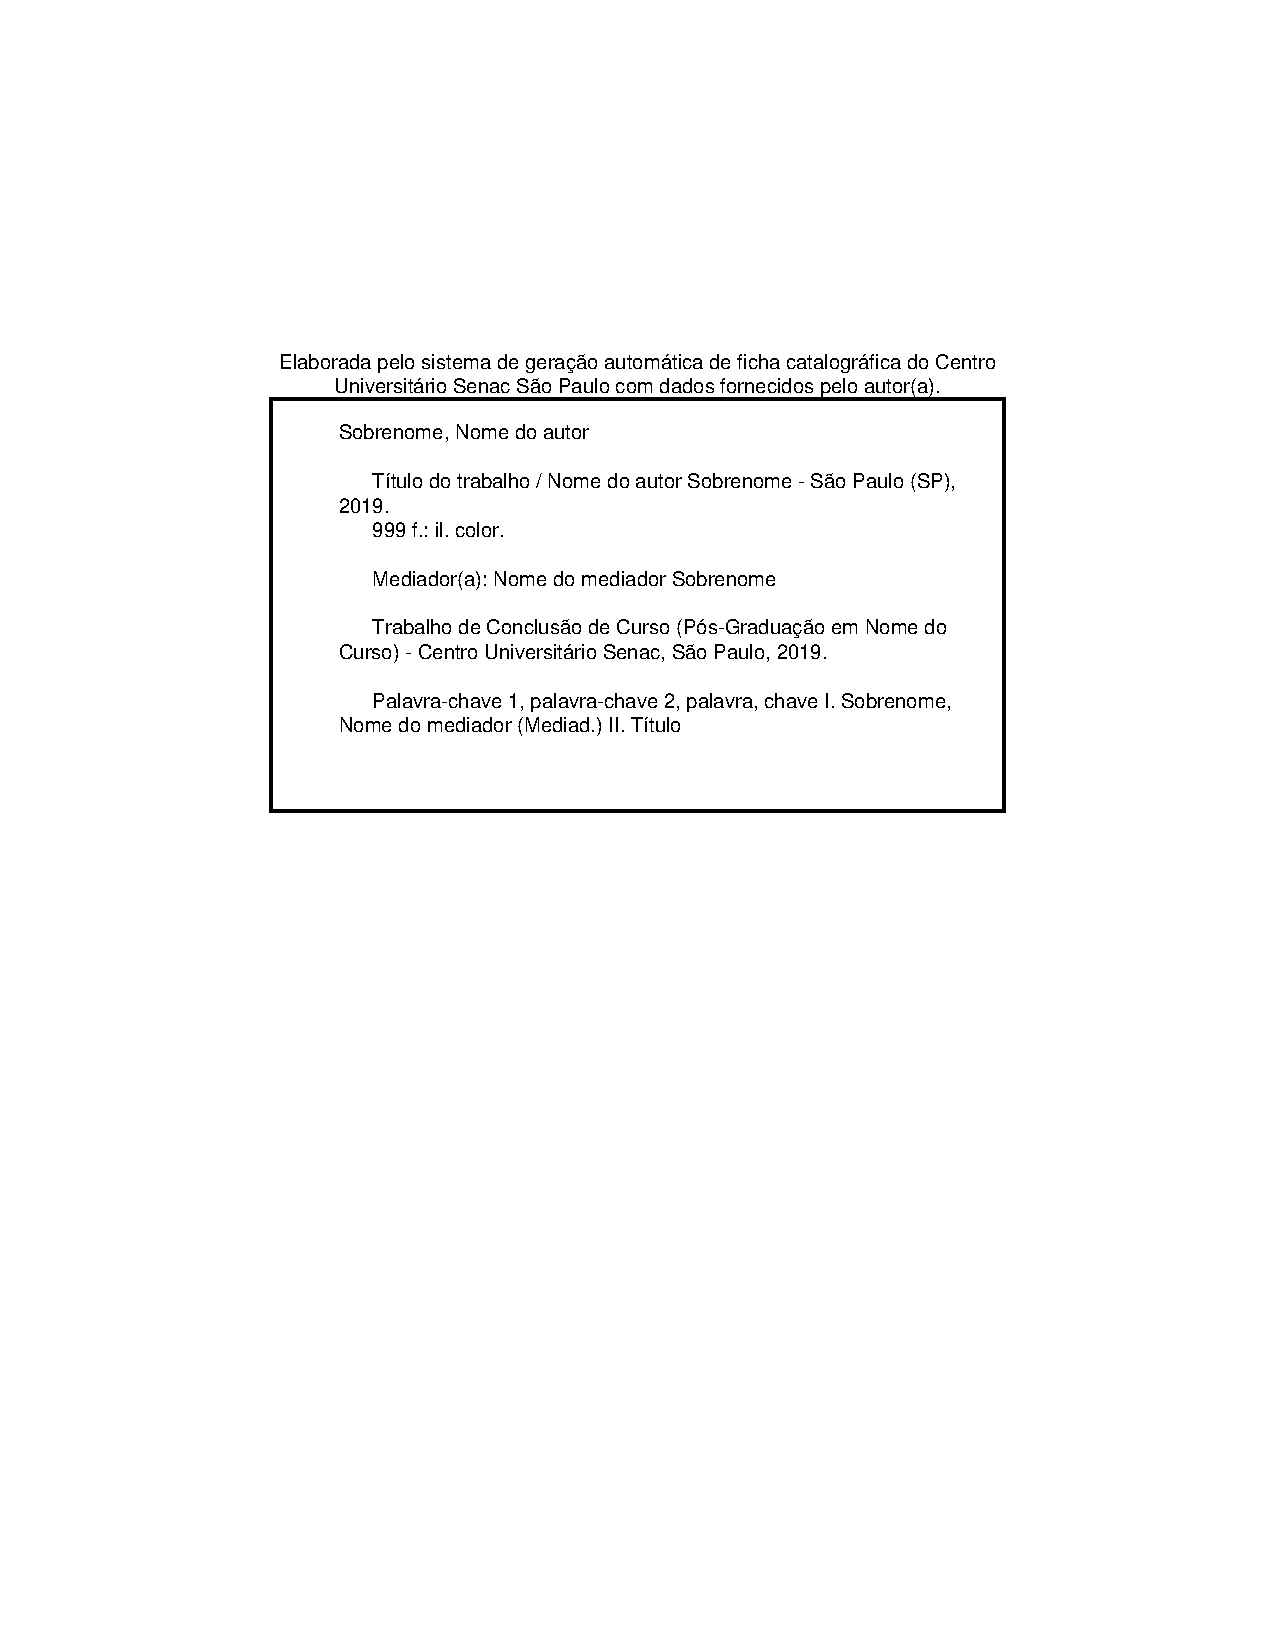
\includepdf{ficha_catalografica.pdf}
\end{fichacatalografica}
% ---

% ---
% Inserir folha de aprovação
% ---
% Isto monta um exemplo de Folha de aprovação, elemento obrigatório da NBR
% 14724/2011 (seção 4.2.1.3). Você pode utilizar este modelo até a aprovação
% do trabalho. Após isso, substitua por uma imagem da página assinada pela 
% banca com o comando abaixo:
%
% \includepdf{folhadeaprovacao_final.pdf}
%
\imprimirfolhadeaprovacaotemporaria
% ---

% ---
% Dedicatória
% ---
\begin{dedicatoria}
   \vspace*{\fill}
   \centering
   \noindent
   \textit{Dedico este trabalho xxxxxxxxx.} \vspace*{\fill}
\end{dedicatoria}
% ---

% ---
% Agradecimentos
% ---
\begin{agradecimentos}
Seus agradecimentos.
\end{agradecimentos}
% ---

% ---
% Epígrafe
% ---
\begin{epigrafe}
    \vspace*{\fill}
	\begin{flushright}
		\textit{``Epígrafe.''\\
		(autor)}
	\end{flushright}
\end{epigrafe}
% ---

% ---
% RESUMOS
% ---

% resumo em português
\setlength{\absparsep}{18pt} % ajusta o espaçamento dos parágrafos do resumo
\begin{resumo}
 \lipsum[1] % substitua por seu resumo

 \textbf{Palavras-chaves}: palavra-chave, palavra-chave, palavra-chave.
\end{resumo}

% resumo em inglês
\begin{resumo}[Abstract]
 \begin{otherlanguage*}{english}
   \lipsum[1] % substitua por seu resumo

   \vspace{\onelineskip}
 
   \noindent 
   \textbf{Keywords}: keyword, keyword, keyword.
 \end{otherlanguage*}
\end{resumo}

% ---
% inserir lista de ilustrações
% ---
\pdfbookmark[0]{\listfigurename}{lof}
\listoffigures*
\cleardoublepage
% ---

% ---
% inserir lista de tabelas
% ---
\pdfbookmark[0]{\listtablename}{lot}
\listoftables*
\cleardoublepage
% ---

% ---
% inserir lista de abreviaturas e siglas
% ---
\begin{siglas}
  \item[EAD] Educação à Distância
  \item[SENAC] Serviço Nacional do Comércio
  \item[TIC] Tecnologia da Informação e Comunicação
  \item[WS] \textit{Web Service}
\end{siglas}
% ---

% ---
% inserir lista de símbolos
% ---
\begin{simbolos}
  \item[$ \Lambda $] Lambda
  \item[$ \mu $] Micro
\end{simbolos}
% ---

% ---
% inserir o sumario
% ---
\pdfbookmark[0]{\contentsname}{toc}
\tableofcontents*
\cleardoublepage
% ---



% ----------------------------------------------------------
% ELEMENTOS TEXTUAIS
% ----------------------------------------------------------
\textual

% ----------------------------------------------------------
% Introdução
% ----------------------------------------------------------
\chapter[Introdução]{Introdução}

\textcolor{red}{Coloque aqui sua introdução.} \lipsum[2]

\section{Tema}

\textcolor{red}{Escreva aqui seu tema -- utilize uma ou duas linhas.}

\section{Justificativa}

\textcolor{red}{Escreva aqui a sua Justificativa -- mais ou menos 2 ou 3 parágrafos.} \lipsum[3-5]

\section{Objetivos}

\subsection{Objetivo geral}

\textcolor{red}{Escreva aqui seu objetivo geral.}

\subsection{Objetivos específicos}

\begin{itemize}
    \item \textcolor{red}{Escreva aqui seu objetivo específico 1;}
    \item \textcolor{red}{Escreva aqui seu objetivo específico 2;}
    \item \textcolor{red}{Escreva aqui seu objetivo específico 3 –- se houver...}
\end{itemize}


\subsection{Problema de pesquisa}

\textcolor{red}{Escreva aqui seu problema de pesquisa -– normalmente um parágrafo.} \lipsum[6]

\subsection{Delimitação do problema de pesquisa}

\textcolor{red}{Escreva aqui sua delimitação do tema de pesquisa – normalmente um parágrafo.} \lipsum[7]

No primeiro capítulo apresenta a Introdução e xxx xxx xx xx.
 	
O segundo capítulo apresenta o Referencial Teórico, detalhando xxxxxxx xxx.
	
O terceiro capítulo apresenta o Referencial Teórico, detalhando outro tópico xxxxxxxxx.

O quarto capítulo apresenta a metodologia de pesquisa. A Metodologia de pesquisa escolhida é a xxx xxx xxxxx e consistirá no Levantamento XXXXX com a revisão da literatura sobre o tema em estudo, além de análise das informações sobre a empresa, objeto deste trabalho.

O quinto capítulo traz a Análise dos Dados xxx x xxxx xxxxx.

No sexto capítulo são apresentadas as Considerações Finais e xxx x x xxx .

Por fim no capítulo sete são apresentadas as Referências xxx x x xxx x xx.

% ----------------------------------------------------------
% REFERENCIAL TEORICO
% ----------------------------------------------------------
\chapter{Um Assunto do Referencial Teórico}

	\textcolor{red}{Revisão da literatura sobre o primeiro conceito ou assunto teórico utilizado (ex: WEB SITES).}
	
	\lipsum[8-9]

\chapter{Outro Assunto do Referencial Teórico}

    \textcolor{red}{Revisão da literatura sobre o segundo conceito ou assunto teórico utilizado (ex: TIPOS DE WEB SITES).}

	\lipsum[10-11]
	
% ----------------------------------------------------------
% METODOLOGIA
% ----------------------------------------------------------
\chapter{Metodologia}

\textcolor{red}{Este capítulo apresenta a metodologia da sua pesquisa.}

\begin{itemize}
    \item Abordagem qualitativa 
    \item Pesquisa bibliográfica
    \item Pesquisa documental (caso utilize dados secundários)
\end{itemize}

Apresentação dos dados secundários (se houver).

O autor \citeonline{mascarenhas_2012} escreveu sobre metodologia científica e está sendo citado aqui apenas para gerar um capítulo de referência bibliográfica mais abaixo. Por falar nisso, aqui vai um exemplo de citação direta longa:

\begin{citacao}
    ``\lipsum[26]
    
    O uso das aspas no Latex é curioso. Não adianta usar o caracter de aspas normais, deve-se iniciar com acento grave duplo e encerrar com duplo apóstrofe.'' \cite[p.~999, texto inventado]{mascarenhas_2012}
\end{citacao}


\lipsum[20]


% ----------------------------------------------------------
% ANÁLISE DOS DADOS
% ----------------------------------------------------------
\chapter{Análise dos dados}

\textcolor{red}{Análise dos dados (relação entre duas abordagens teóricas ou de teoria x dados) exemplo: relacionar os tipos de teste identificados no capitulo 3 com as tecnologias apresentadas no capitulo 2. Aqui devem ser apontadas as relações entre os fatos investigados e a teoria que lhes dá respaldo. Por exemplo: discutir se utilizar teste de sql injection é mais efetivo em plataformas Windows ou Linux ou em linguagens como ruby on rails, asp.net ou java.}

\lipsum[12-13]

% ----------------------------------------------------------
% CONSIDERAÇÕES FINAIS
% ----------------------------------------------------------
\chapter{Considerações Finais}

\textcolor{red}{Nesse ponto deverão ser evidenciados os objetivos alcançados com a pesquisa (resgatando–os da sua introdução – vide item 1.3.2), indicando as limitações encontradas no desenvolvimento do trabalho e os possíveis desenvolvimentos futuros.}

\lipsum[14-15]

% ----------------------------------------------------------
% Finaliza a parte no bookmark do PDF
% para que se inicie o bookmark na raiz
% e adiciona espaço de parte no Sumário
% ----------------------------------------------------------
%\phantompart

% ----------------------------------------------------------
% ELEMENTOS PÓS-TEXTUAIS
% ----------------------------------------------------------
\postextual
% ----------------------------------------------------------

% ----------------------------------------------------------
% Referências bibliográficas
% ----------------------------------------------------------
\bibliography{referencias}

% ----------------------------------------------------------
% Glossário
% ----------------------------------------------------------
%
% Consulte o manual da classe abntex2 para orientações sobre o glossário.
%
%\glossary

% ----------------------------------------------------------
% Apêndices
% ----------------------------------------------------------

% ---
% Inicia os apêndices
% ---
\begin{apendicesenv}

% Imprime uma página indicando o início dos apêndices
%\partapendices

% ----------------------------------------------------------
\chapter{Modelo de Questionário Aplicado na Pesquisa}
% ----------------------------------------------------------

\textcolor{red}{Se você utilizou, por exemplo, um questionário para a realização da pesquisa, o modelo utilizado deverá ser colocado neste capítulo como APÊNDICE.}

\lipsum[50]

% ----------------------------------------------------------
\chapter{Cronograma}
% ----------------------------------------------------------

O quadro a seguir apresenta a cronologia prevista para as principais etapas do desenvolvimento deste Trabalho de Conclusão de Curso.

%\begin{quadro}[htb]
%\caption{\label{quadro_cronograma}Cronograma das etapas do trabalho}
\vskip\baselineskip
\noindent
\begin{tabularx}{\linewidth}{|X|c|}
\hline
\textbf{Etapa} & \textbf{Período previsto} \\ \hline
1. Definição do tema de pesquisa, metodologia e referenciais iniciais & até nov/2018 \\ \hline
2. Aprofundamento do estudo de referenciais teóricos & dez/2018 a fev/2019 \\ \hline
3. Levantamento de dados	& jan-mar/2019 \\ \hline
4. Aplicação de questionários & mar-abr/2019 \\ \hline
5. Tabulação de dados & abr-jun/2019 \\ \hline
6. Análise de dados & jun-out/2019 \\ \hline
7. Elaboração das conclusões/considerações finais & nov-dez/2019 \\ \hline
8. Revisão e entrega final do TCC & jan/2020 \\ \hline
9. Preparação e realização da defesa/prova final & jan-fev/2020 \\ \hline
\end{tabularx}
\fonte{Autor.}
%\end{quadro}

Este cronograma é um instrumento de planejamento da elaboração deste TCC e não constará na versão final.

\end{apendicesenv}
% ---


% ----------------------------------------------------------
% Anexos
% ----------------------------------------------------------

% ---
% Inicia os anexos
% ---
\begin{anexosenv}

% Imprime uma página indicando o início dos anexos
%\partanexos

% ---
\chapter{Tabelas de Dados XPTO}
% ---

\textcolor{red}{Caso tenha utilizado no TCC tabelas de dados, cálculos, etc, deverá inserir os dados como ANEXO.}

\lipsum[30]

\end{anexosenv}

%---------------------------------------------------------------------
% INDICE REMISSIVO
%---------------------------------------------------------------------
%\phantompart
\printindex
%---------------------------------------------------------------------

\end{document}
